\documentclass[11pt]{article}

\usepackage[strings]{underscore}
\usepackage{amsmath}
\usepackage{graphicx}
\usepackage{amssymb}
\usepackage{mathspec}
\usepackage{geometry}
\usepackage{placeins}
\usepackage{graphicx}

\geometry{a4paper, portrait, margin=1in}
\DeclareMathOperator*{\argmax}{arg\,max}

\begin{document}

\section*{Q1}
\subsection*{Part 1}
See Code.

\subsection*{Part 2}
See Code.

\subsection*{Part 3}
See Code.

\subsection*{Part 4}
French: 1308 tokens

\noindent English: 1279 tokens

\noindent Training Samples: 8701 sentences between en/fr

\noindent Batch Size: 32

\noindent Batches/Epoch: 272

\noindent Epochs: our model ran for 50 epochs and did not early stop.

\bigskip

\noindent Training perplexity is reported every 320 samples or 10 batches. Dev perplexity is reported every 3200 samples or 100 batches. It seems both training and dev
perplexity do fall although slower over time. See Figure~\ref{fig:ppl}. It seems the gains after a few dozen iteration sets are not very significant.

\begin{figure}
  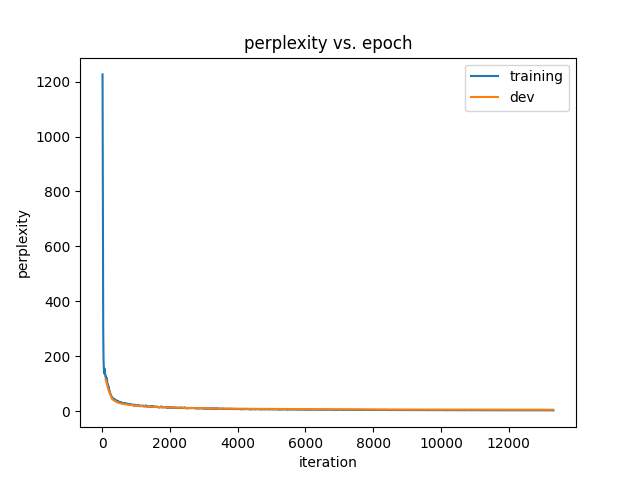
\includegraphics[scale=0.5]{pplfigure.png}
  \caption{Training Iterations vs. (Dev, Training) Perplexity}
  \label{fig:ppl}
\end{figure}

\bigskip

\noindent The translation of the dev set from english to french has a BLEU score of 39.32 (higher the better).
The quality of the translation is rather poor, but the fluency seems to be okay on the dev set.
There seems to be significant errors for words that have been Byte Pair Encoded (BPE .e.g., @@ words).

\section*{Q2}

\subsection*{Part 1}

The BLEU score with different decoder (128) and encoder (64) hidden layer sizes is 34.17.

\subsection*{Part 2}

The BLEU score for additive attention is 42.00.

\bigskip

\noindent The BLEU score for dot-product attention is 38.89.

\subsection*{Part 3}

Architectural changes include stacking more layers into the LSTM. There are also many other forms of attention. Also maybe ReLu-ing some
of the hidden layer projections (not sure intuitively why this helps, but yolo). And I guess you can always go transformers!

\bigskip

\noindent In terms of improvements to speed, the early stopping probably can be improved along with a better set of hyper-parameter search. Also
another mechanism is to optimize using a difference kind of loss (dunno what off the top of my head) or another dev metric other than perplexity.

\bigskip

\noindent The training algorithm iterates until either early stopping or until max epoch. It computes loss first by summing the loss along the
sequence dimension (returned by model.forward()) in var \textit{example_losses}. Then it is batch summed into a cumulative loss that is then
divided by the batch size to get the average cumulative loss across the sentences, which then backpropagation occurs
so the update weights is an average across the batch. Avg Loss is the loss across batches and Avg Perplexity is the exponential of that loss. 
Early stopping is checked every var \textit{rgs.valid\_niter} times, where the metric perplexity is used where the cumulative loss across all
dev words is divided by the number of words to translate. If a better model based on the metric is found it is saved to model.bin and model.bin.optim
and patience count reset. Otherwise patience count is incremented for this dev evaluation. If patience count hits a limit, then this trial path is given up
on if no improvement was found and num_trials incremented. If num_trials hit a args.max\_num\_trials then early stopping is triggered. If a
trial path is given up on, learning rate decay is triggered on the optimizer and the model is reloaded from the best found at the start when patience=0.

\bigskip

\noindent Decode loads the model from the saved model.bin and model.bin.optim parameters along with the test target and src sentences and
vocab. It calls beam search and extracts the top most likely hypotheses sentence to compare to the target sentence. It uses the nltk corpus_bleu
function to calculus a BLEU score form 0-100 with lower the better. 

\bigskip

\noindent The beam search decoding algorithm can be found in \textit{nmt\_model.py} beam_search function. In this function it uses the trained
model parameters for the encoding and embedding layer to first create the inputs to the decoder. Then the beam search takes it step by step,
creating beam search width number of sentences each time. A sentence ends either via `</s>` token or hitting the maximum number of tokens
allowed. The current set of completed hypothesis sentences are kept in the var \textit{completed\_hypothesis} and the log\_prob score of such a
sentence is tracked in var \textit{hyp_scores} while the current sentences are tracked in list[list[]] var \textit{hypothesis}. In calculating the top K
next words, the current scores in \textit{hyp\_scores} is expanded to the length of the vocab and the output log probabilities of the vocab is then
broadcast-added to the \textit{hyp\_scores} from which the top K words is found in the matrix (K x words so far) using torch.topk(...). This is why
the next operations are an integer division to figure out the root index of the sentence so far and a remainder operation to figure out the new word.
The next hidden and cell states after the initial '<s>' token is a batch (K x hidden\_size) which is fished out by the var \textit{live\_hyp\_ids} (which
of the K hidden states from decoder step is the topk choice to use as \textit{prev\_hyp\_id} in the next iteration). 

\section*{Q3}

\subsection*{Part 1}
\subsubsection*{A}
The downside of maximizing over $\Sigma_{(w,c) \in D} log(\frac{e^{v_c \cdot u_w}}{\Sigma_{c^{'} \in V} e^{v_{c^{'}} \cdot u_w}})$ is that the corpus $V$ can be really large
and this can be computationally expensive as the denominator is over all V rather than just select words N. Also it feels as if this loss function favours overfitting of the
word embeddings.

\subsubsection*{B}
Yes, ideally the more likely words that appear more often that do not appear in the context would be more likely to be chosen. If an uniform distribution is applied, some more
likely words would get closer to the target word as it becomes less likely to be chosen as negative samples and words that appear less will be further away from the target word as it would be
more likely to be chosen as negative samples . It feels like this would not be as a representative language model (underfitting). 

\subsection*{Part 2}
The larger the context window, the more costly the computation as there are more context words to optimize over to update the hidden vector. But more importantly, a context
window of 1 basically means that there is no context. A context window of 5 means we understand the features of a sentence and context window of 100 means we may
extrapolate the features of a paragraph.

\subsection*{Part 3}
With this smoothing distribution, the unigram frequency distribution becomes more uniform for $\alpha<0$ and less uniform for $alpha>0$. A more uniform distribution leads to
underfitting and is a form of regularization. The similarity with most words will decrease as the rare words would be more likely to be chosen as negative samples to optimize away from
then the words they are in the context for which would optimize them close to some other words (there are more words not in rare words' context, than there are words in rare words' context). 

\subsection*{Part 4}
The similarity can be rewritten as:

\begin{align}
	\begin{split}
	cos(y, b-a+x) = cos(y,b) - cos(y,a) + cos(y,x)
	\end{split}
\end{align}

\noindent It may be that $cos(y,b) - cos(y,a) \approx 0$ as London and England occur pretty simultaneously in the same context and with only Baghdad as the input, then similar words that
co-occur in similar context may not be necessarily Iraq but other Iraqi cities. 

%\section*{Q1}
%
%What you want to construct is an OR gate based on previous and current values. It is sufficient to consider the base case at $t0 \rightarrow t1$ and the case for
%$t1 \rightarrow t2$. The rest follows by induction. At time step 1 we must satisfy two equations:
%
%\begin{align}
%	\begin{split}
%		h_1 &= f( w_1 + b_2 ) \;\;\;\; for \; x_1 = 1 \\
%		y_1 &= 1 = x_3h_1+b_3 \\
%		h_1 &= f(b_2) ];\;\;\; for \; x_1 = 0 \\
%		y_1 &= 0 = x_3h_1+b_3
%	\end{split}
%\end{align}
%
%\noindent For this case, we can choose $b_2 > 0$ or $b_2 \leq 0$. In the latter case, this creates a contradiction where $w_1 + b_2 > 0$ and $w_1 + b_2 \leq 0$
%simultaneously. Therefore we choose $b_2 > 0$. This implies the following:
%
%\begin{align}
%	\begin{split}
%		b_3 &= 1 \\
%		x_3 &= -1 \\
%		w_1+b_2 &\leq 0 \\
%		b_2 &> 0	
%	\end{split}
%\end{align}
%
%Working on the system of equations for $t1 \rightarrow t2$ given that $h_1=0$ for $x_1=1$ and $h_1=1$ for $x_1=0$:
%
%\begin{align}
%	\begin{split}
%		h_2 &= f(b_2) \;\;\;\; for \; x_1 = 1, x_2 = 0 \\
%		y_2 = 0 &= x_3h_2 + b_3 \\
%		h_2 &= f(w_1+b_2) = 0 \;\;\;\; for \; x_1=1, x_2=1 \\
%		y_2 = 1 &= b_3 = 1 \\
%		h_2 &= f(w_2+b_2) \;\;\;\; for \; x_1=0, x_2=0 \\
%		y_2 = 0 &= x_3h_2+b_3 \\
%		h_2 &= f(w_1+w_2+b_2) \;\;\;\; for \; x_1=0, x_2=1 \\
%		y_2 = 0 &= x_3h_2+b_3 
%	\end{split}
%\end{align}
%
%\noindent This creates the following implications:
%	
%\begin{align}
%	\begin{split}
%		b_2 &> 0 \\
%		w_1+b_2 &\leq 0 \\
%		w_2+b_2 &> 0 \\
%		w_1+w_2+b_2 &> 0  \\
%		b_3 &= 1 \\
%		x_3 &= -1 \\
%		b_2 &= 1 \\
%		w_1 &= -1 \\
%		w_2 &= 1
%	\end{split}
%\end{align}
%
%\section*{Q2}
%
%Using the same reasoning as above, you can establish similar set of constraints:
%\begin{align}
%	\begin{split}
%		b_2 &\leq 0 \\
%		w_1+b_2 &> 0 \\
%		w_2+b_2 &\leq 0 \\
%		w_1+w_2+b_2 &> 0  \\
%	\end{split}
%\end{align}
%
%\noindent The solution for these constraints are:
%
%\begin{align}
%	\begin{split}
%		b_3 &= 1 \\
%		x_3 &= -1 \\
%		b_2 &= 0 \\
%		w_1 &= 1 \\
%		w_2 &= 0
%	\end{split}
%\end{align}
%
%\noindent Which interestingly removes the concurrent feedback path in the RNN.
%
%\section*{Q3}
%
%Highest weighted unigrams (-): 
%
%\begin{quote}
%('too', tensor(0.4642)), ('bad', tensor(0.4078)), ("n't", tensor(0.3311)),
%
%('no', tensor(0.3101)), ('dull', tensor(0.2750)), ('worst', tensor(0.2291)), 
%
%('minutes', tensor(0.2126)), ('plot', tensor(0.2024)), ('mess', tensor(0.1895)), 
%
%('flat', tensor(0.1803))              
%\end{quote}
%
%\noindent Least weighted unigrams (-): 
%
%\begin{quote}
%('funny', tensor(-1.3329)), ('most', tensor(-1.1824)), ('best', tensor(-1.1650)), 
%
%('love', tensor(-1.1536)), ('story', tensor(-1.0664)), ('about', tensor(-1.0500)), 
%
%('performances', tensor(-0.9468)), ('life', tensor(-0.8979)), ('who', tensor(-0.8322)), 
%
%('work', tensor(-0.8290))
%\end{quote}
%
%\noindent Highest weighted unigrams (+):
%
%\begin{quote}
%('best', tensor(0.4150)), ('fun', tensor(0.3577)), ('love', tensor(0.3464)), 
%
%('heart', tensor(0.3055)), ('entertaining', tensor(0.2991)), ('fascinating', tensor(0.2743)), 
%
%('world', tensor(0.2416)), ('solid', tensor(0.2404)), ('documentary', tensor(0.2351)), 
%
%('us', tensor(0.2328))
%\end{quote}
%
%\noindent Least weighted unigrams (+): 
%
%\begin{quote}
%("n't", tensor(-3.2279)), ('too', tensor(-2.1348)), ('or', tensor(-1.7833)),
%
%('like', tensor(-1.7680)), ('bad', tensor(-1.5712)), ('no', tensor(-1.3889)),
%
%('just', tensor(-1.3437)), ('more', tensor(-1.1376)), ('much', tensor(-1.0718)),
%
%('does', tensor(-1.0701))
%\end{quote} 
%
%\section*{Q4}
%
%\begin{table}
%	\begin{center}
%		\begin{tabular}{l|c|c|c|c|}
%		\textbf{Epoch} & \textbf{Training Accuracy} & \textbf{Dev Accuracy} \\
%		\hline
%		0 & 0.68916 & 0.7236  \\
%		1 & 0.7459 & 0.7201 \\
%		2 & 0.7579 & 0.7190  \\
%		3 & 0.7610 & 0.7202 \\
%		4 & 0.7638 & 0.7201 \\
%		5 & 0.7653 & 0.7202\\
%		6 & 0.7658 & 0.7202 \\
%		7 & 0.7657 & 0.7202 \\
%		8 & 0.7660 & 0.7202 \\
%		9 & 0.7666 & 0.7202 \\
%		10 & 0.7664 & 0.7202 \\
%		11 & 0.7673. & 0.7202 \\
%		12 & 0.7676 & 0.7202 \\
%		13 & 0.7680 & 0.7202 \\
%		14 & 0.7675 & 0.7202 \\
%		15 & 0.7680 & 0.7202 \\
%		16 & 0.7670 & 0.7202 \\
%		17 & 0.7682 & 0.7202 \\
%		18 & 0.7674 & 0.7202 \\
%		19 & 0.7683 & 0.7202 \\
%		\end{tabular}\
%		\caption{Unigram Model - Epoch 20, Learning Rate 0.001}
%		\label{tbl:unigram}
%	\end{center}
%\end{table}
%                                                                                                                                                                                                                                 
%I do not think with greater epochs the dev accuracy will improve. It seems, since my unigram model does not contain prefix or suffix features, it cannot generalize at all to unseen words. Further there
%are certain unigram words that require context to decide whether it is (+) or (-) which overfits in the training data set. Also more than a few epochs doesn't seem to help as the parameter updates are
%purely additive or subtractive on the same training set, which only accentuates the overfitting as time goes on, especially against unseen data in the dev set. The table of the epoch is shown in Table~\ref{tbl:unigram}.
%
%\section*{Q5}
%
%Too lazy to matplotlib or table-fy the result in latex, so here it is, you can see the performance dramatically improves in both training and dev with bigram and trigram models that incorporates <UNK>
%token. I also added L2 regularization.
%
%epoch 0: train acc = 0.6885838150289018, dev acc = 0.7419724770642202
%
%epoch 1: train acc = 0.8197976878612717, dev acc = 0.7603211009174312
%
%epoch 2: train acc = 0.875578034682081, dev acc = 0.7626146788990825
%
%epoch 3: train acc = 0.903757225433526, dev acc = 0.7660550458715596
%
%epoch 4: train acc = 0.9215317919075144, dev acc = 0.7706422018348624
%
%epoch 5: train acc = 0.9338150289017341, dev acc = 0.7729357798165137
%
%epoch 6: train acc = 0.9442196531791908, dev acc = 0.7672018348623854
%
%epoch 7: train acc = 0.95, dev acc = 0.7752293577981652
%
%epoch 8: train acc = 0.9578034682080925, dev acc = 0.7821100917431193
%
%epoch 9: train acc = 0.9627167630057804, dev acc = 0.783256880733945
%
%epoch 10: train acc = 0.9661849710982658, dev acc = 0.786697247706422
%
%epoch 11: train acc = 0.9684971098265895, dev acc = 0.7935779816513762
%
%epoch 12: train acc = 0.9703757225433526, dev acc = 0.7958715596330275
%
%epoch 13: train acc = 0.9738439306358382, dev acc = 0.7981651376146789
%
%epoch 14: train acc = 0.9761560693641619, dev acc = 0.7993119266055045
%
%epoch 15: train acc = 0.977456647398844, dev acc = 0.7970183486238532
%
%epoch 16: train acc = 0.9787572254335261, dev acc = 0.7970183486238532
%
%epoch 17: train acc = 0.9799132947976879, dev acc = 0.7970183486238532
%
%epoch 18: train acc = 0.982514450867052, dev acc = 0.7970183486238532
%
%epoch 19: train acc = 0.9832369942196532, dev acc = 0.7981651376146789 
%
%\section*{Q6}
%
%A basic feed-forward linear neural network was implemented. It seems that some learning is happening and it does perform
%better than the unigram model. 
%
%epoch 0: train acc = 0.7270231213872832, dev acc = 0.7534403669724771
%
%epoch 1: train acc = 0.7614161849710983, dev acc = 0.7729357798165137
%
%epoch 2: train acc = 0.7705202312138728, dev acc = 0.7752293577981652
%
%epoch 3: train acc = 0.7697976878612717, dev acc = 0.7603211009174312
%
%epoch 4: train acc = 0.7721098265895954, dev acc = 0.7637614678899083
%
%epoch 5: train acc = 0.7797687861271676, dev acc = 0.75
%
%epoch 6: train acc = 0.7791907514450868, dev acc = 0.7603211009174312
%
%epoch 7: train acc = 0.7807803468208092, dev acc = 0.75
%
%epoch 8: train acc = 0.7771676300578034, dev acc = 0.6961009174311926
%
%epoch 9: train acc = 0.7836705202312139, dev acc = 0.7557339449541285
%
%\section*{Q7}
%
%The improvement over the unigram model is significant and it seems to even surpass the hand-tuned ngram features of the perceptron
%classifier. It does see to be overfitting, so adding some dropout (0.2) to the RNN could be useful (currently 0).
%
%epoch 0: train acc = 0.7732658959537573, dev acc = 0.805045871559633
%
%epoch 1: train acc = 0.8543352601156069, dev acc = 0.819954128440367
%
%epoch 2: train acc = 0.8947976878612717, dev acc = 0.8142201834862385
%
%epoch 3: train acc = 0.9290462427745665, dev acc = 0.8188073394495413
%
%epoch 4: train acc = 0.9606936416184971, dev acc = 0.8188073394495413
%
%epoch 5: train acc = 0.9773121387283237, dev acc = 0.8061926605504587
%
%epoch 6: train acc = 0.9851156069364162, dev acc = 0.8084862385321101
%
%epoch 7: train acc = 0.9891618497109826, dev acc = 0.8038990825688074
%
%epoch 8: train acc = 0.9920520231213873, dev acc = 0.8119266055045872
%
%epoch 9: train acc = 0.9927745664739884, dev acc = 0.7855504587155964
%
%\section*{Q8}
%
%Skipped. I assume you can figure out how to implement this with a multi-layered transformer where the input are your GloVe vectors (with different sentence length padded). On the output, you just
%look at a single sigmoid-ed output. Just have to figure out how to do the loss with tensorflow or pytorch, which will require reading the documentation and look up examples on the Google.
%
%Alternatively you can improve the RNN, see the comments in the code for \textit{MyNNClassifier} in \textit{model.py}.

\bibliographystyle{abbrv}
\bibliography{solutions}

\end{document}
